\documentclass[../00_main.tex]{subfiles}

\begin{document}

\section{Python Satellite Data Program}

This section details how to setup and use the program and how it works.
First, the setup is discussed and then each of the successive stages are
detailed. The information about different functions and ways to use Python and
the libraries are taken from the documentation. Because many different
libraries and elements work together, I will not point out every single one but
name the required one here.
% TODO: put all the libraries here

\subsection{Setup}

The programs and data required to use the program are the following:
\begin{itemize}
    \item netCDF data files (preferably from M2I3NPASM because it has been
        tested),
    \item a working installation of the Anaconda Python distribution (available
        \href{https://www.anaconda.com/products/individual}{here}).
\end{itemize}
Then one has to get the code to the program and set up the required anaconda 
environment. The code can either be downloaded from my Github repository which
can be found \href{https://github.com/moritz-konarski/internship}{here}, or I 
can provide it upon request. \\
Setting up the anaconda environment is simple.
Navigate to the \texttt{programs} folder in my internship repository. Then,
open that folder in a terminal (it must be \texttt{cmd.exe} on windows,
Powershell will not work). In the terminal, type \texttt{conda env create
--file internship\_gui.yml} (on Windows, use \texttt{conda env create
--file internship\_gui\_win.yml}). This command will create a Python
environment with all the required dependencies for my program. The installation
might take a while. The resulting environment
will have the same name as the file it was created from. To use the environment
is has to be activated with \texttt{conda activate internship\_gui} (or 
\texttt{conda activate internship\_gui\_win}. Once the environment is
activated, navigate to the \texttt{gui\_program} folder. To execute the
program, run the command \texttt{python3 main.py} (\texttt{python main.py} on
Windows). You should see a window that looks like \figref{dp01}.
\begin{figure}[H]
    \center
    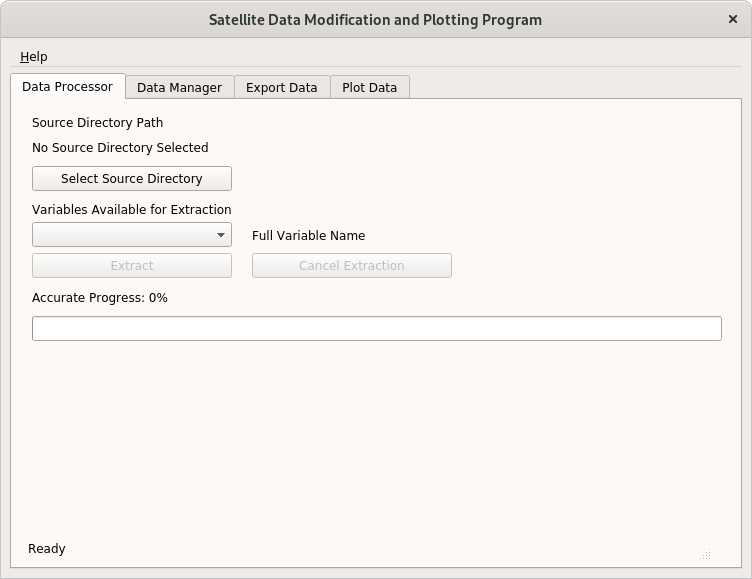
\includegraphics[width=0.75\textwidth]{../graphics/dp01}
    \caption{The Data Processor Tab}
    \label{dp01}
\end{figure}

\subsection{Data Processing}

The first screen of the program is the Data Processor as seen in \figref{dp01}.
The purpose of the Data Processor is to take netCDF files as input, extract
a single variable from them and save it to a NPZ file. It is made up of two
classes, the \texttt{DataProcessor.py} class, a \texttt{QThread} that performs the
processing, and the \texttt{DataProcessorTab.py} class which handles the UI. 
The steps to using it are the following:
\begin{enumerate}
    \item Click the \textbf{Select Source Directory} button. An input dialog
        (\figref{dp02})
        will appear where you will have to select the folder where the netCDF
        files are located. The validity of the specified directory will be
        checked. 
            \begin{figure}[H]
                \center
                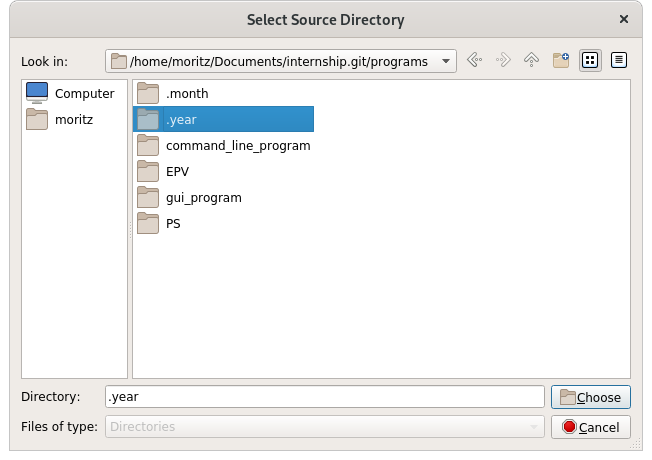
\includegraphics[width=0.75\textwidth]{../graphics/dp02}
                \caption{The Source Directory Selection Popup}
                \label{dp02}
            \end{figure}
    \item After \textbf{Choose} is clicked, the directory is checked to
        make sure it actually contains netCDF files. Then, the available
        variables are extracted from the first file. They are displayed in
        a drop-down list in their short form and then the selected one's
        full name is displayed (see \figref{dp03}). Here the user must 
        choose one of the variables to extract. 
        \begin{figure}[H]
            \center
            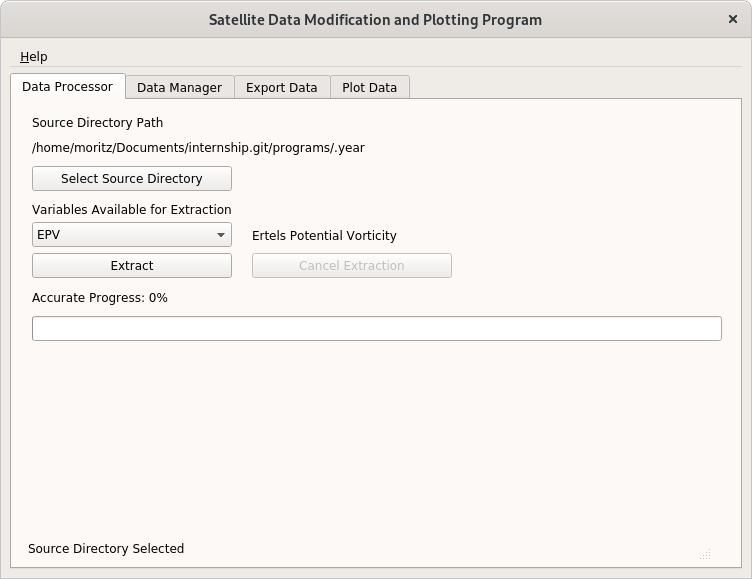
\includegraphics[width=0.75\textwidth]{../graphics/dp03}
            \caption{Data Processor with loaded source Directory}
            \label{dp04}
        \end{figure}
    \item When the choice is made, click \textbf{Extract}. A popup asking
        for a destination directory will appear where the user should
        indicate where the files should be saved. In case the extraction
        takes too long or the user changes their mind, the \textbf{Cancle
        Extraction} button will stop the extraction process. \figref{dp04}
        shows the extraction process.
        \begin{figure}[H]
            \center
            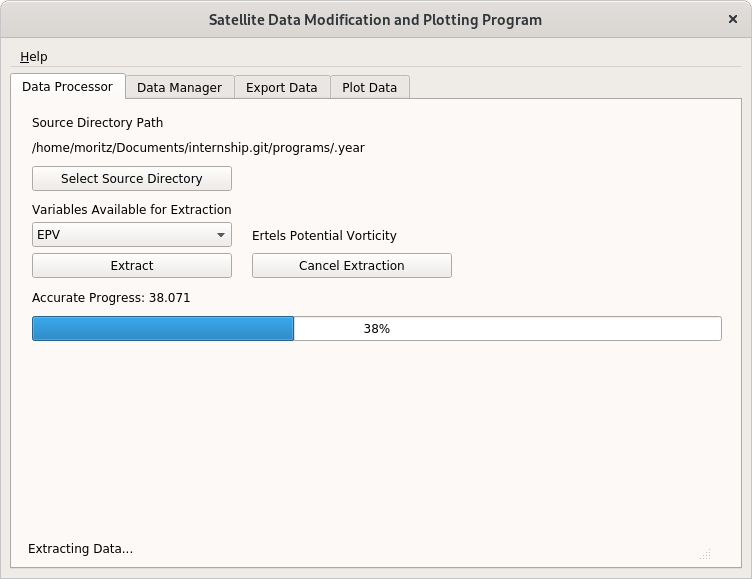
\includegraphics[width=0.75\textwidth]{../graphics/dp04}
            \caption{Extraction in Progress}
            \label{dp04}
        \end{figure}
\end{enumerate}
This process will create a new directory in the directory the user selected.
This directory will be named after the short name of the variable. It will
contain the NPZ file named \texttt{<short variable name>.npz}, which
will contain all the relevant data, and a file called
\texttt{metadata.json}, which contains all the important metadata information
that was contained in the netCDF file.\\ 
Once the extraction process is complete, the user can either continue using
this program and switch to the Data Manager tab, or take the created folder and
use the NPZ file with any \texttt{numpy}--compatible program.

\subsection{Data Management}

\begin{figure}[H]
    \center
    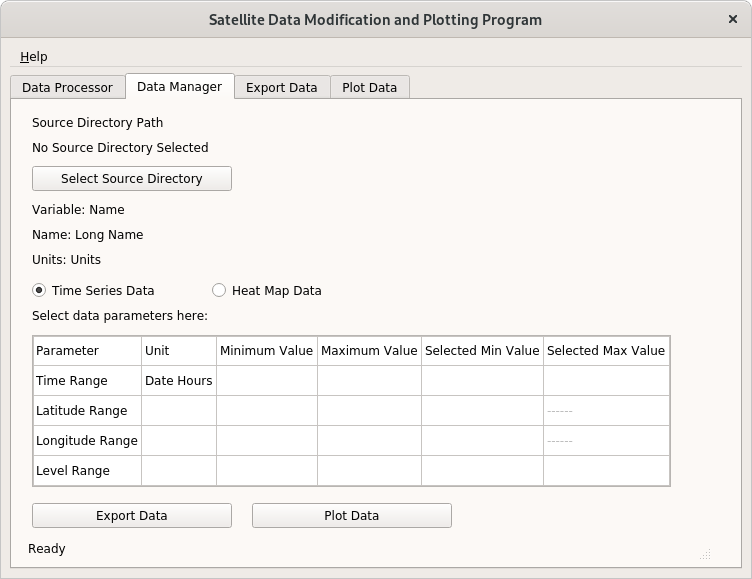
\includegraphics[width=0.75\textwidth]{../graphics/dm01}
    \caption{The Data Manager Tab}
    \label{dm01}
\end{figure}

The Data Manager seen in \figref{dm01} is responsible for selecting the data 
subset the user intends to use and the type of data the user intends to use.
The data subset is defined by setting minimum and maximum values for the
dimensions of the data. The type of data is either a time series, where
a location is fixed and all data for that point is available, or a heat map
where a range of latitude and longitude is selected and then all data for that
is selection is used. The Data Manager, much like the Data Processor, has two
parts, the \texttt{DataManager.py}, responsible for providing the data, and the
\texttt{DataManagerTab.py}, which is responsible for the GUI. The Data Manager
is used like this:
\begin{enumerate}
    \item Click the \textbf{Select Source Directory} button. An input dialog
        will appear where you will have to select the folder that was created
        by the Data Processor (the validity of the folder will be checked).
    \item After the directory has been successfully selected, the variable
        name, long variable name, and the unit of the variable will be
        displayed. Furthermore, the table at the bottom will be filled in with
        the minimum and maximum values that are available according to the file
        that was provided. \figref{dm02} illustrates this step.
        \begin{figure}[H]
            \center
            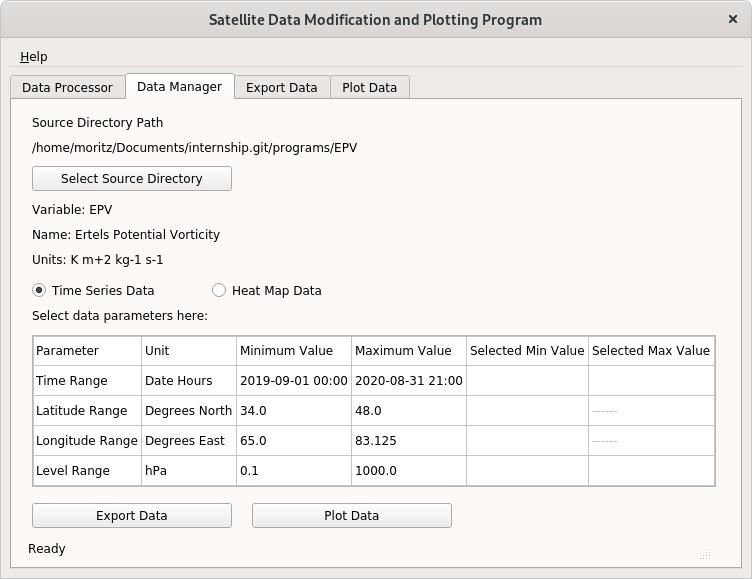
\includegraphics[width=0.75\textwidth]{../graphics/dm02}
            \caption{Data Manager with loaded Directory}
            \label{dm02}
        \end{figure}
    \item With the directory selected, the user now needs to choose the limits
        of the data dimensions by entering them into the table. All user
        input will be validated and in case a value is outside of the possible
        values, an error message is shown. Furthermore, all entered values will
        automatically be corrected to the closest available value. The radio
        buttons determine if time series data (see \figref{dm03}) or heat map 
        data (see \figref{dm04}) is selected and
        the table is adjusted accordingly. If the selected data does not have
        a level associated with it, the last row of the table is disabled (see
        \figref{dm05}).
        \begin{figure}[H]
            \center
            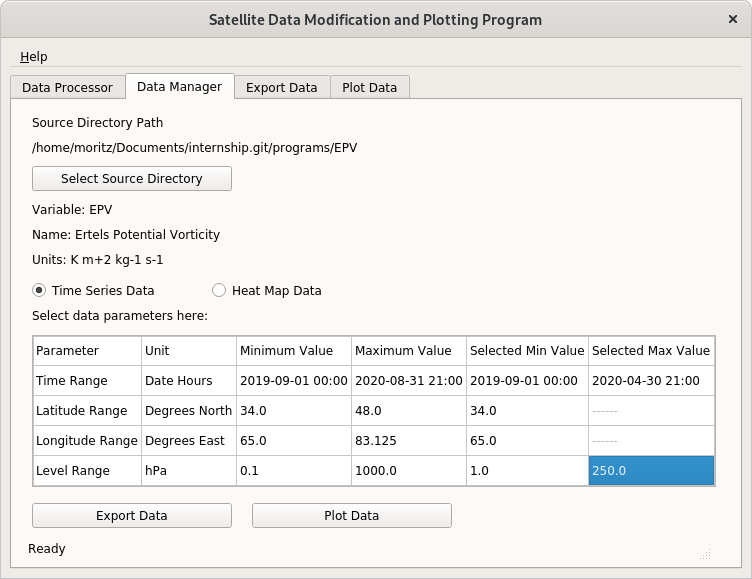
\includegraphics[width=0.75\textwidth]{../graphics/dm03}
            \caption{Data Manager in Time Series Mode}
            \label{dm03}
        \end{figure}
        \begin{figure}[H]
            \center
            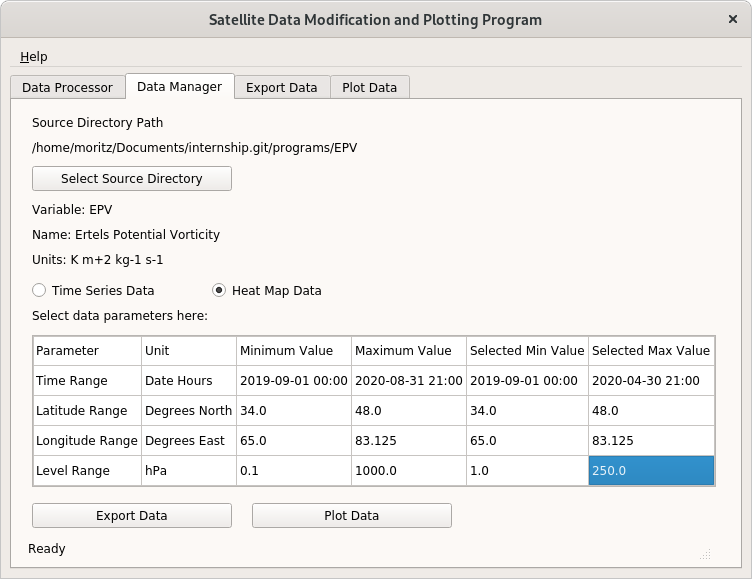
\includegraphics[width=0.75\textwidth]{../graphics/dm04}
            \caption{Data Manager in Heat Map Mode}
            \label{dm04}
        \end{figure}
        \begin{figure}[H]
            \center
            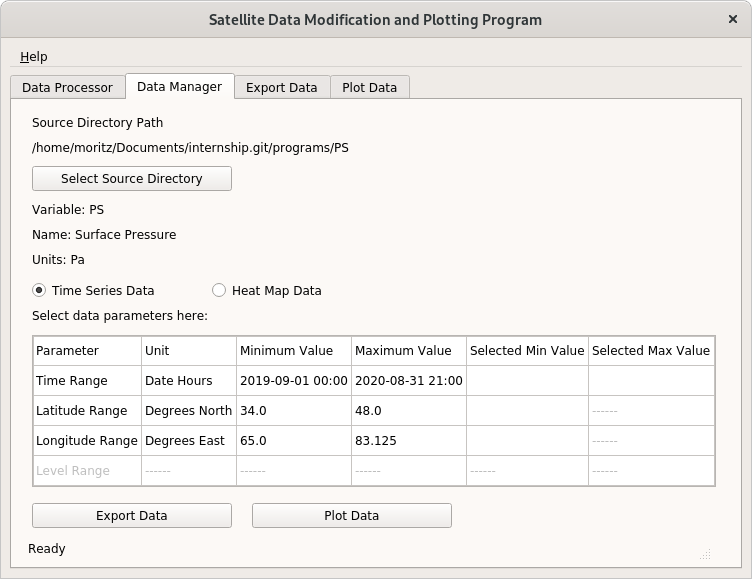
\includegraphics[width=0.75\textwidth]{../graphics/dm05}
            \caption{Data Manager with data without level}
            \label{dm05}
        \end{figure}
    \item When all data fields have been filled, the user may either press the
        \textbf{Export Data} button or the \textbf{Plot Data} button. Each of
        the buttons will prepare the associated data and then switch to the
        corresponding tab.
\end{enumerate}
The value entered in the Data Manager are persistent, meaning that if the user
exports some data first and then wants to plot the same data, they only need to
go back to the Data Manager tab and press \textbf{Plot Data}.

\subsection{Data Exporting}

\subsection{Data Plotting}

\subsection{Help}

\end{document}
